\chapter{Introduction}\label{chp:chp1}

%\begin{flushright}
%  {\em QUOTE GOES HERE }\\
%
%\ \
%
%\normalsize
%{AUTHOR}  
%\end{flushright}


\noindent{Should you choose to seek out one of my friends and ask them about my whereabouts in recent months,
%acquaintances and to enquire of them my whereabouts in recent months
 %they would likely stare at you blankly.  Upon further interrogation 
 they would probably yield the information that I had been noticeable by my absence because I was preoccupied writing about dust, a fact which I imagine they  find bemusing and possibly somewhat concerning.  Blissful as they are in their ignorance of dust (astronomers find no such peace), they do not know the importance of this all-pervading substance.}

The universe is an extremely dusty place.  The ubiquity of dust throughout almost all epochs and environments demands a comprehensive understanding of its formation and evolution, properties and effects.  It plays numerous roles in a variety of scenes; it is a building block of  all solid bodies, a birthing place for molecules, a crucial ingredient in star formation and an extreme annoyance for cosmologists.  It is both a product of physical processes and an agent of chemical ones.

It is perhaps confusing therefore that there is comparatively little consensus regarding the formation processes and natal environments that result in the evolution of certain atoms and molecules into the grains we call dust.  Over the years since the first discovery  of dust in the very early universe, a growing population of astronomers and astrophysicists have turned their attention to the study of dust formation in core-collapse supernovae (CCSNe), in the hope that these objects might prove to be the missing piece of the puzzle.  Recent observations of a number of CCSNe and supernova remnants (SNRs) have lent weight to this theory, with models and analyses of spectral energy distributions (SEDs)  suggesting the presence of large reservoirs of cool, ejecta-condensed dust in these objects. 

I have sought to make my own contribution to this field by exploiting a different observational signature, that of  blue-shifted line profile asymmetries observed in the spectra of many CCSNe and attributed to the formation of dust in the ejecta.  By quantitatively modelling these characteristically asymmetric line profiles using a new code, DAMOCLES, I have attempted to determine the rate of dust formation in CCSNe and the expected order of magnitude of the eventual dust masses produced.

Throughout the remainder of this chapter I will attempt to elucidate the above synopsis in more detail.  In Section \ref{scn:dust}, a brief description of the roles that dust plays in the universe will be followed by a discussion of the physical properties of dust that allow for its detection in emission and absorption.  In Section \ref{scn:ccsne}, I will give a summary of our current understanding of dust formation, with particular attention paid to dust formation in CCSNe.  At the end of this section, I will describe the current state of the field before concluding this chapter
% with a short justification of the approach that I have adopted for this work and 
with an outline of the aims and structure of this thesis.


\section{A Handful of Dust}
\label{scn:dust}

\subsection{A Brief History}

The presence of dust in the universe was first theorised when astronomers observed dark patches of sky in the Milky Way where all of the stars had been ``erased" (see Figure \ref{intro:fig:dustpatch}).  Whilst some claimed that these black regions were in fact a true absence of stars resulting from some anomaly in the stellar distribution, others felt that it was more likely that an obscuring cloud of material was blocking the light from the stars behind.  In 1930, Donald \citeauthor{Trumpler1930} confirmed this latter theory by considering the apparent magnitudes and colours of stars located at different angles to the galactic plane, discovering that those closer to the plane appeared redder than their more distant counterparts \citep{Trumpler1930}.  This was the first evidence of interstellar reddening and the beginnings of our understanding of dust as a scatterer, absorber and emitter of radiation.

For the next few decades, dust was largely thought to be  an irritating obstacle to observing and comprehending more interesting facets of the universe.  We now have a much fuller understanding of the variety and importance of the roles that dust plays throughout astrophysics.

\begin{figure}
\centering
\includegraphics[scale=0.7]{chapters/chapter1/figs/black_patch_B68.jpg}
\caption{The dark globule Barnard 68, LDN 57.  ESO press release 30 April 1999.}
\label{intro:fig:dustpatch}
\end{figure}

\subsection{The Roles of Dust in the Universe}

Despite comprising only $\sim$1\% of the mass of the interstellar medium (ISM), dust grains account for as much as 30\% of the total galactic luminosity via their emission in the infra-red (IR) \citep{Li2003}.  In the cycle of matter from the ISM to condensing clouds to stars and back again, dust is far more than a passive passenger along for the ride.  Whilst residing in the ISM, dust is important in determining its thermodynamics.  It acts both as a heating agent via the emission of photoelectrons in regions of strong ultra-violet (UV) radiation and a coolant in dense regions via the emission of IR radiation.  In this role as a coolant, dust is also crucial to the process of star-formation, helping to remove gravitational energy and allowing the natal cloud to collapse.  Dust also contributes to the star formation process by shielding the gas from ionising radiation, helping to speed up the growth of the protostellar core. 

In addition to the above physical functions, dust plays an essential part in chemical processes.  Dust grains  attract gaseous atoms to their surfaces and catalyse the formation of molecules, which are then released back into the surrounding medium.  The chemistry of the ISM is also altered by the inclusion of metals in dust grains which causes a general depletion of heavy elements.

Dust does not reside solely in the ISM however.  It is present in  large quantities in the circumnuclear tori found around active galactic nuclei.  Dust is also found between planets, around stars and in protoplanetary discs, where dust grains constitute the smallest unit of the building blocks that  go on to form planetesimals and planets.  These grains may even be responsible for the origins of life.  

The more detailed our understanding of dust as an astrophysical community, the more accurate we can make our inferences across an entire range of  fields.  There is arguably no other topic in astronomy that has such wide-ranging effects.


\subsection{The Medium of Dust}
\label{scn:dust_med}
%\subsubsection{Composition}

An increasingly detailed knowledge of the nature and properties of dust has developed over the last few decades. Dust grains have their terrestrial analogue in soot or very fine sand rather than in the dust bunnies that one may find behind the sofa.  When found in the ISM they are generally small, between 0.05\micron\ and 0.25\micron\ in radius, and are normally predominantly composed of carbon or silicates.  Carbonaceous grains may take many forms ranging from structured solids such as diamond and graphite to amorphous molecules and aromatics.  They are generally found to be strongly attenuating.  Silicates tend to be more glassy and contain silicon and oxygen potentially with the dirtying addition of magnesium, iron or other heavier elements.  Condensates of more complex molecules such as olivine (MgFeSiO$_4$) and pyroxene (MgSiO$_3$) make up these grains.  Whilst our understanding of the chemical and physical facets of dust is ever improving, there are still a number of largely unresolved issues.  %regarding the makeup of a dusty medium.

Dust grains are generally assumed to be spherical in order to make their simulative treatment more straightforward but in reality dust grain shapes are actually much more complex.  Sophisticated models of dust grains sometimes adopt a continuous distribution of ellipsoids to represent dust grain shape \citep{Bohren1983}.  This distribution allows grains to take any ellipsoidal form ranging from flat discs to needles to perfect spheres.  However, even this more detailed consideration omits structures that are akin to long strings or to fluffy particles (see Figure \ref{dust_grain}). Heretofore, the  majority of models, including DAMOCLES, have generally only considered spherical grains.  The wide variety of grain morphologies therefore represents a significant modelling challenge to be addressed in the future.



Different species and composites thereof have different optical properties i.e. those properties of a dust grain that determine the nature of its interaction with radiation.  In order to model the absorption and scattering of radiation by dust grains, it is first necessary to know the complex refractive indices of the species of interest over the relevant wavelength range (see Sections \ref{opt_prop} and \ref{scn:mie_theory}).  Laboratory measurements have produced a number of different sets of optical constants for a variety of carbonaceous and silicate species and these are well-utilised throughout the field \citep{Draine1984,Zubko1996,Jager2003}.  It is noted at this early juncture however that in many cases there are numerous, somewhat contradictory, sets of optical constants for a given species and that these variations can potentially cause a degree of confusion regarding the results of models that use them \citep{Owen2015}.  
%This topic will be discussed in detail later in this thesis (SECTION).
%Dust in the universe follows a cycle.  From its stellar birthplace, it is ejected and slowly integrates itself with the ISM before condensing into molecular clouds and ultimately once again returning to stars.  Most of the knowledge of the properties of dust applies only to grains in the ISM, which are found to follow a grain radius distribution $n(a) \propto a^{-3.5}$ as described by \citeauthor{Mathis1977} in 1977.  This distribution does not necessarily apply immediately after their formation, however, as grains are subject to numerous forces that can result in their destruction, sputtering or evaporation.  The grain size distribution and relative abundances of species of newly-formed grains are still topics in dispute and are issues that I attempt to address in my models.  The issue of dust grain shape will hopefully be addressed in future versions of DAMOCLES (see Section \ref{limitations}).
%
%\section{The Physics of Dust}



\subsection{Optical Properties of Dust}
\label{opt_prop}


%This paragraph used to introduce the physics of dust section
In order to quantitatively model the effects of dust on line emission in an expanding atmosphere, the physics of how dust particles scatter, absorb and re-emit radiation must be understood. In the next few sections, I will review the physical aspects of dust grains that allow for their detection via emission in the IR and absorption and scattering in the UV and optical.   

\begin{figure}
\centering
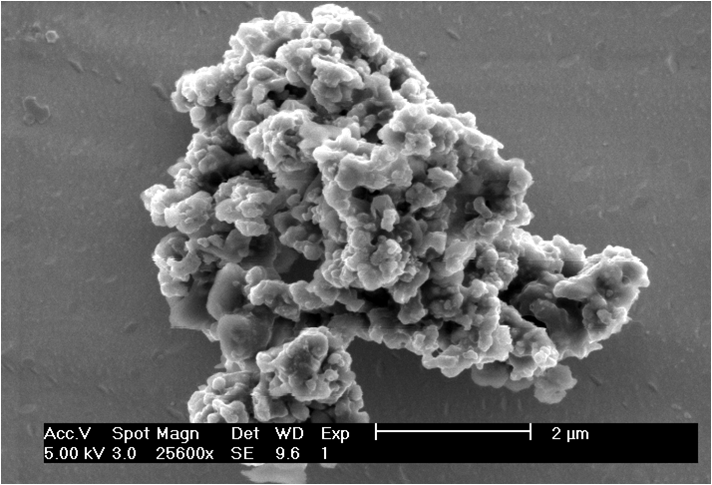
\includegraphics[scale=0.5]{chapters/chapter1/figs/dust_grain.png}
\caption{A typical ``fluffy" chondritic porous IDP composed of nanometre-sized mineral grains and organic matter. (Credit: N. Spring).}
\label{dust_grain}
\end{figure}

%In order to be able to model the effects of a medium of dust grains on a dynamic radiation field, 
We must first be able to describe the manner in which a single dust grain scatters an incident photon and with what probability it will absorb rather than scatter that photon. These properties are defined via the scattering and absorption cross-sections of interaction ($C_{sca}$ and $C_{abs}$ respectively).  In combination with the scattering anisotropy parameter $g$, they are used to define the angular distribution and amount of  light that is scattered by the grain.  The aim is to calculate these quantities for a beam of radiation of given wavelength, incident on a particle of given size and shape, and composed of a given material.   

Calculation of these quantities is not straightforward.  In order to determine the above properties, we must take a step back to first principles, away from dust, and consider what is meant by `scattering' and `absorption'.  Matter, regardless of its superficial composition, is intrinsically composed of fundamental, charged particles: electrons and protons.  When an electromagnetic field is induced in the presence of these particles, such as when a beam of radiation illuminates an obstacle, which could be a liquid or an atom or a dust grain or a solid, the fundamental particles that make up that object are set into oscillatory motion.  These motions cause the radiation of electromagnetic energy and it is this secondary radiation that we refer to as scattered light.  Similarly, the excited charges may transform some of the incident energy into other forms such as thermal energy.  This is the process that is referred to as absorption.

Returning now to the concept of scattering and absorption by a single particle, derivation of the quantities of interest, namely $C_{sca}$ and $C_{abs}$, requires us to be able to describe the electromagnetic field at all points interior to and exterior to the particle.  In order to perform this calculation, we imagine that the particle is made up of infinitesimally small regions each of which is approximated as a dipole in the presence of an applied oscillating field (i.e. an incident electromagnetic photon).  The strength of the applied electromagnetic field affects that strength of the response by each of the dipoles and thus of the dust grain as a whole.  The relationship between this response and the induced field is determined by the material, which is described for this purpose by the complex refractive index 
\begin{equation}
m(\lambda)=n(\lambda)+ik(\lambda)
\end{equation}

\noindent where $n(\lambda)$ and $k(\lambda)$ are the real and the imaginary parts of the complex refractive index.  Broadly speaking, $n$ may be considered to describe the scattering component of the complex refractive index and $k$ the absorptive component.  These optical properties are the starting point to solving Maxwell's equations inside and outside of the particle and thus calculating the scattering and absorption cross-sections.

\subsection{Mie Theory}
\label{scn:mie_theory}

Whilst relatively simple approximations to this calculation exist in the regime where the scattering particle is substantially smaller than the wavelength (the Rayleigh regime), for particles which are of a similar size to the wavelength of the incident radiation, the calculation is a complex one.  The full solution to Maxwell's equations in this case was first described by Gustav Mie in 1908 \citep{Mie1908}.  The Mie solution has wide application to a number of fields ranging from the study of interstellar dust to plasmonics.  Mie himself developed his approach in order to better understand the colourful effects of a colloidal gold solution.  The nature of Mie's solution meant that it was not widely used until many years after its initial publication, when computing power had reached a stage capable of computing the infinite series expansions on which the solution depends.

In this section, I will discuss the key results that allow for the calculation of the scattering and absorption efficiencies that are crucial for modelling the effects of dust on electromagnetic radiation.  Much of this mathematics is somewhat dense and I will therefore restrict my discussion to the most relevant points. An outline of the derivation of  Mie's solution to Maxwell's equations is given in Appendix \ref{append:appendA}.  For further details and an unusually lyrical description of the relevant physics and mathematics please see \citet{Bohren1983}, on which the majority of this section and Appendix \ref{append:appendA} are based.  

For my models, the wavelength of the monochromatic line to be modelled is very often of a similar order of magnitude to the grain radius and as such the full Mie solution must be implemented.  %I describe the approach to this solution in some detail (although the rather laborious algebra is largely omitted) in Appendix \ref{append:appendA}.  
For a single spherical particle, the scattering cross-section of interaction, $C_{sca}$, is defined to be the net rate at which electromagnetic energy is scattered across the surface of the particle divided by the total irradiance of the incident beam (i.e. the rate at which energy falls onto the surface).  The extinction cross-section, $C_{ext}$, is similarly defined.  

For a spherical particle of radius $a$ and an incident beam of wavelength $\lambda$, we may define the size parameter
\begin{equation}
x=\frac{2\pi N a}{\lambda}
\end{equation}

\noindent where $N$ is the complex refractive index of the surrounding medium.  Assuming the particle to be surrounded by a vacuum such that $N=1$, we can show that the scattering coefficients are given by 
\begin{align}
a_n &= \frac{m\psi_n(mx)\psi_n'(x)-\psi_n(x)\psi_n'(mx)}{m\psi_n(mx)\xi'_n(x)-\xi_n(x)\psi'_n(mx)} \\[2ex]
b_n &= \frac{\psi_n(mx)\psi_n'(x)-m\psi_n(x)\psi_n'(mx)}{\psi_n(mx)\xi'_n(x)-m\xi_n(x)\psi'_n(mx)}
\end{align}


\noindent where $m$ is the complex refractive index of the particle and a prime denotes differentiation with respect to the argument in parentheses. The scalar functions $\psi_n$ and $\xi_n$ are the Ricatti-Bessel functions and are given by
\begin{equation}
\psi_n(\rho) = \rho j_n(\rho) \, , \quad \quad \xi_n(\rho)=\rho h_n^{(1)}(\rho)
\end{equation}

\noindent where $j_n$ and $h_n^{(1)}$ are the spherical Bessel functions of the first and second kind.  The scattering coefficients can then be used to calculate the scattering and extinction cross-sections of interaction:
\begin{align}
C_{sca}&=\frac{2\pi}{\tilde{k}^2}\sum_{n=1}^{\infty} (2n+1)(|a_n|^2+|b_n|^2) \\
C_{ext}&=\frac{2\pi}{\tilde{k}^2}\sum_{n=1}^{\infty} (2n+1)\textnormal{Re}\{a_n+b_n\} 
\end{align}

\noindent where $\tilde{k}$ is the wavevector and {\em not} the imaginary component of the refractive index $m$.  For a single spherical particle of radius $a$, the scattering and extinction efficiencies are related to the interaction cross-sections via
\begin{equation}
Q_{ext}=\frac{C_{ext}}{\pi a^2}\, , \quad \quad Q_{sca}=\frac{C_{sca}}{\pi a^2}
\end{equation}

\noindent We can therefore calculate the extinction and scattering cross-sections given the wavelength of the incident photon and the optical properties of the dust grain.  



The above solution has the primary drawback of only being applicable to spherical particles although there are extensions to more complex morphological distributions such as the ``T-matrix method" and the ``Discrete Dipole Approximation" \citep{Mishchenko2002,Draine2004}). Obviously, the adoption of the original Mie solution presents a potential issue for a medium of dust grains that may well be crystalline, fluffy or extremely amorphous (see Figure \ref{dust_grain}).  However, despite its limitations, Mie theory does provide a first-order description of the optical effects of non-spherical particles.  DAMOCLES adopts the Mie theory solution to Maxwell's equations in order to calculate scattering and absorption efficiencies.  In the future, when alternative morphologies may be considered, the algorithm may be extended to alternative solutions  in order to address this limitation.  Similarly, the above solution applies only to a single particle.  Various weighted summations must be performed over the scattering and extinction cross-sections in order to treat a medium of multiple different grain sizes and species.  This is discussed in further depth in Sections \ref{scn:grainsize} and \ref{gs_distn}.

Having established the physics behind light scattering and extinction by dust grains, I can now consider how the effects of dust on radiation manifest themselves in observations. 

\begin{figure}
\centering
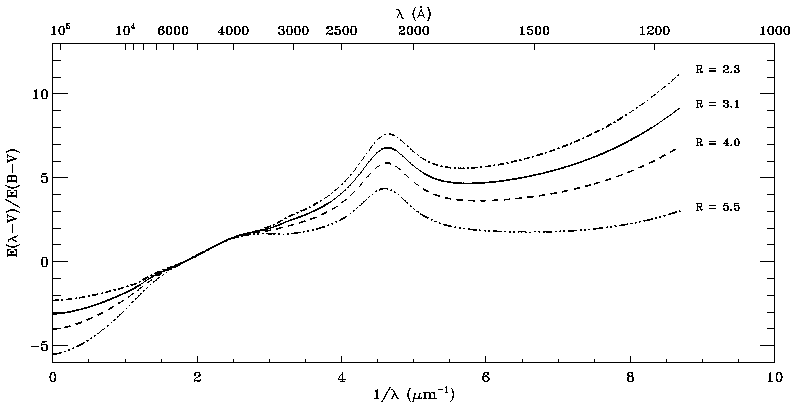
\includegraphics[clip=true,scale=0.53,trim= 0 0 0 0]{chapters/chapter1/figs/extinction_curves2.png}
\caption{Extinction curves for different values of $R_V$ across the UV, optical and IR based on the parametrisation by \citet{Cardelli1989}.  The bump at 2175\AA\ can be clearly seen in all curves.}
\label{fig:ext_curve}
\end{figure}

\subsection{Dust in Absorption}
\label{scn:abs}
 

We may relate the frequency-dependent extinction cross-section to the opacity $\kappa_{\nu}$ of the dusty medium via
\begin{equation}
\kappa_{\nu} \rho = C_{ext,\nu} n_d
\end{equation}
\noindent where $n_d$ is the number density of the dust, $\rho$ is the mass density and $\nu$ is the frequency.  The opacity determines the fraction of radiation that is absorbed when a beam of given frequency travels through the medium.  It also determines the continuum emission of the dust as we shall see in Section \ref{scn:emission}.  The intensity of the beam after having travelled a distance $x$ is given by
\begin{equation}
I(x)=I_0 e^{-\kappa_{\nu} \rho x}
\end{equation}
\noindent  for a medium with constant density $\rho$ and initial intensity $I_0$.  The optical depth  is defined to be the quantity $\tau_{\nu}=\kappa_{\nu} \rho x$.  This relationship is clearly central to understanding the effects of dust absorption on line profiles emitted in the ejecta of CCSNe.  However, it applies to any dusty environment.  The ISM in particular has proved to be central to developing our understanding of dust and much of what we now know is the result of investigations into the attenuating effects of dust in the ISM.  
 
By considering the reddening and attenuation of starlight from background stars,  \citet{Bless1972} determined the first section of the interstellar extinction curve from 0.11$\mu$m to 2.15$\mu$m.  Eventually, further observations would allow for the variation of interstellar extinction to be determined across the full wavelength range \citep{Rieke1985}.  It was found that dust in the ISM is most strongly attenuating at shorter wavelengths and its extinction efficiency decreases towards the IR, with a noticeable bump at around 2175\AA\ (see Figure \ref{fig:ext_curve}). This prominent feature of the extinction curve is a result of the chemical makeup and optical properties of the dust that resides in the interstellar medium, although its precise origin remains unknown.  In 1989, \citeauthor*{Cardelli1989} postulated that not only was the total interstellar extinction (from the UV to the NIR) independent of the line-of-sight to the background stars, but that it could be entirely characterised by the quantity
\begin{equation}
R_V=\frac{A_V}{A_B-A_V}=\frac{A_V}{E(B-V)}
\end{equation}
\noindent $A_V$ and $A_B$ represent the extinction in the V- and B-bands respectively. The quantity $R_V$ is known as the {\em total-to-selective} extinction.  The extinction in the ISM can generally be described by $R_V\approx3.1$ whilst denser regions such as some molecular clouds are described by $R_V\approx5$.  Properties of the ISM extinction curve, such as the strong absorption feature seen at around 10$\mu$m, allowed \citet*{Mathis1977} to determine the composition and grain size distribution of dust in the ISM.  They attributed the 10$\mu$m absorption feature to silicates and found that a grain size distribution $n(a) \propto a^{-3.5}$, with graphite grains distributed between $0.001<a<1\mu$m and silicate grains distributed between $0.025<a<0.25\mu$m, would reproduce the extinction curve.  This grain size distribution has become known as the ``MRN" distribution as a result.    A figure illustrating the variation of extinction with wavelength at longer wavelengths clearly showing the 10$\mu$m feature is given in Figure \ref{fig:extinction_curve_10um} \citep{Weingartner2001,Draine2003}.

%\begin{figure}
%\centering
%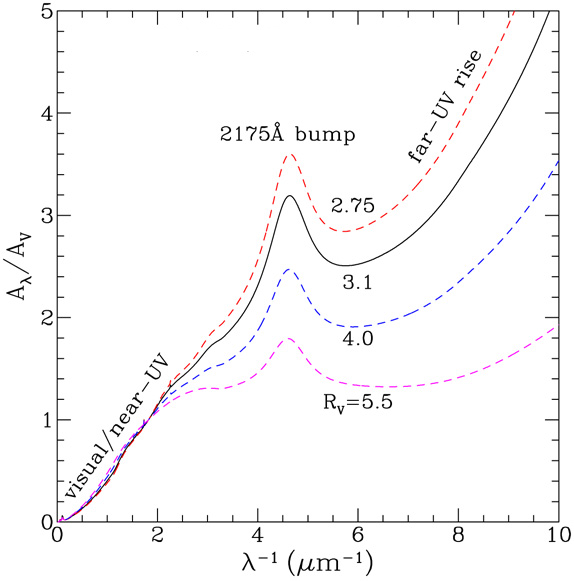
\includegraphics[clip=true,scale=1,trim= 0 0 0 0]{chapters/chapter1/figs/extinction_curves.png}
%\caption{Extinction curves for different values of $R_V$ across the UV, optical and IR based on the parametrisation by \citet{Cardelli1989} .  The bump at 2175\AA\ can be clearly seen in all curves.}
%\label{fig:ext_curve}
%\end{figure}

\begin{figure}
\centering
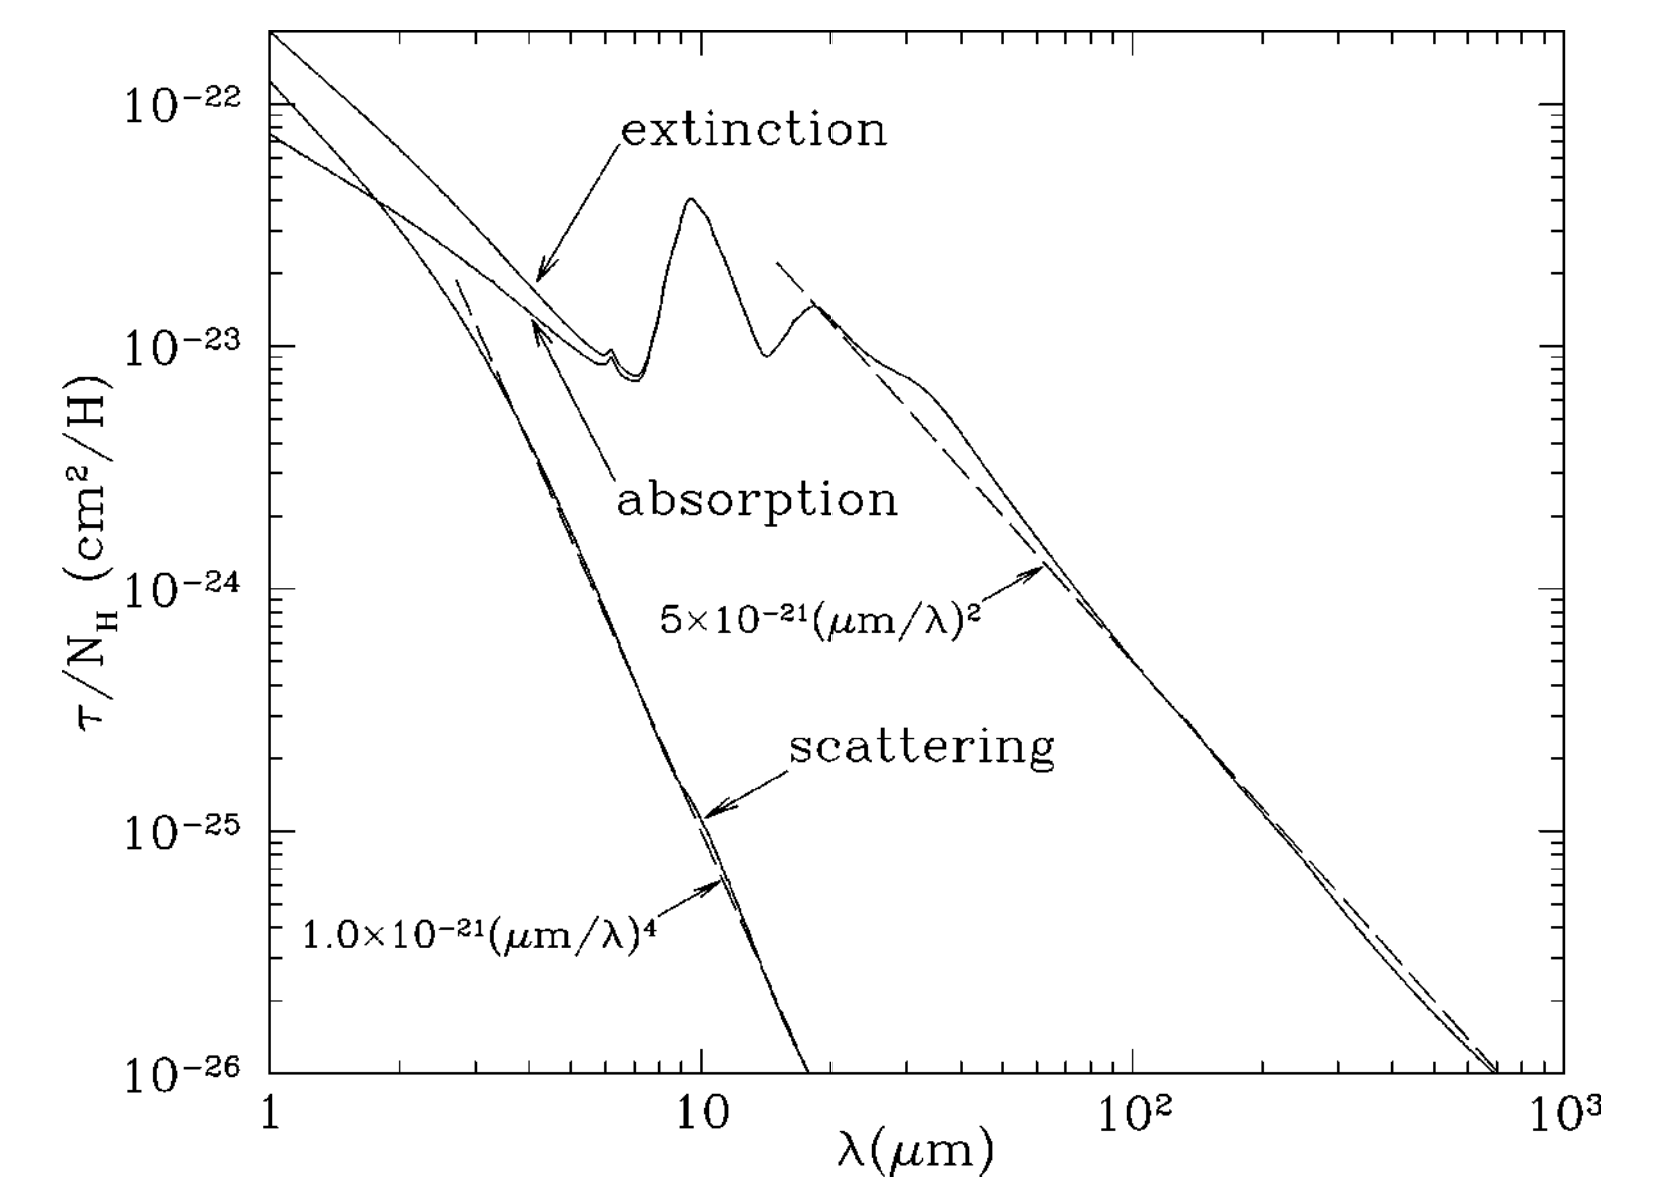
\includegraphics[clip=true,scale=0.43,trim= 0 0 0 0]{chapters/chapter1/figs/extinction_curve_10um.png}
\caption{Extinction curves for  $R_V=3.1$ at short wavelengths as calculated by  \citet{Draine2003} using the model of \citet{Weingartner2001}.  The 10$\mu$m absorption feature can be clearly seen.}
\label{fig:extinction_curve_10um}
\end{figure}

\subsection{Dust in Emission}
\label{scn:emission}
Energy absorbed by dust grains in the optical and UV causes the dust to be heated.  Warm dust emits continuum radiation in the near- to mid-IR and cool dust emits in the far-IR and sub-millimetre (sub-mm).  For dust that is in local thermodynamic equilibrium in an optically thin environment, the continuum emission from the dust, $F_{\nu}$,  is proportional to the temperature-dependent blackbody spectrum, $B_{\nu}(T)$ \citep{Hildebrand1983}:
\begin{equation}
F_{\nu}\propto \kappa_{\nu} B_{\nu}(T)
\end{equation}

\noindent This expression determines the temperature dependence of dust grains with a given opacity. Using this relationship, it is possible to fit theoretical SEDs to  observed photometric data in the IR and sub-mm in order to derive various properties of the emitting dust, such as the dust mass and composition.  It is usually this approach that is employed to determine dust masses in various objects from observations.  For a single component, the temperature and opacity are iterated over until the SED best-fits the observed data points and then these properties are translated to a dust mass via the optical properties of the dust as discussed in the previous sections.  Often the size distribution of the dust grains and the composition are also considered as variables, and a multi-component fit that allows for the presence of dust at different temperatures is frequently adopted to obtain a  more realistic fitting.  In order to fit  the full range of the SED from the optical to the sub-mm without assumptions of single temperature components  a fully self-consisted radiative transfer model must be employed (see Section \ref{scn:rt}).

In addition to its continuum emission, dust also has a number of spectroscopic emission features.  These features allow the composition of dust in a given region to be probed more directly than is possible using SED fitting.  A detailed discussion of the spectroscopic features of a variety of dust species ranging from silicates to ices is given by \citet{Draine2003}. 
%do i need to go into detail on spectroscopic features of dust???  Seems unlikely...

\subsection{Dust as a Scatterer}

Dust's role as a scatterer is not often considered and has few observable signatures.  However, it gives rise to some particularly unusual and interesting features in the fast moving environments of supernovae.  As shall be discussed in detail throughout this thesis, dust scattering can result in significant, possibly asymmetrical broadening of emission lines and the appearance of an extended scattering wing on the red side of the profile \citep{Lucy1989}. 

 It can also cause an effect known as a ``light echo".  This is when light emitted from an object is reflected off a surrounding dusty region, such as a dense circumstellar shell, back towards the observer. Observing light echoes allows astronomers to see the state of an object in the past and therefore to understand its evolution.  Analysis of light echoes from Cassiopeia~A (Cas~A) allowed its age and SN type to be determined \citep{Krause2008} and the circumstellar environment of SN~1987A was investigated using light echoes as well \citep{Sugerman2005}.  Whilst light echoes can provide much insight into the past, they can also present a problem for current observations.  When observing supernovae, it is important to determine whether observations are of the current state of the object or a previous one.

\subsection{Radiative Transfer in Dusty Media}
\label{scn:rt}
In Section \ref{scn:abs}, I discussed the effect of dust absorption on an incident beam of radiation.  In general, the calculation of the emergent radiation field given an incident field on a dusty medium is not a straightforward one.  This calculation is dependent on the {\em equation of radiation transfer}.  This equation defines the relationship between an incident beam of radiation and the emergent beam based on the properties of the medium through which it is passing.  Mathematically, it is given by 
\begin{equation}
\label{eqn:rt}
\frac{dI_{\nu}}{ds}=\rho \kappa_{\nu} I_{\nu} + \rho j_{\nu}
\end{equation}
 
\noindent where $\nu$ is the frequency of the beam and $I_{\nu}$ is the intensity of the beam.  The quantity $j_{\nu}$ is the emission coefficient per unit mass and determines the radiated emission.  The quantity $s$ represents distance and as such $\frac{dI_{\nu}}{ds}$ is the rate of change of the intensity of the beam with distance.  All other quantities are as previously defined.  The first term in Equation \ref{eqn:rt} represent the absorption by the dust and the second term represents emission along the line $ds$, as well as light that is scattered into the path of the beam.

In certain cases, this equation can be solved analytically.  However, for general cases and particularly for complex 3-dimensional geometries, it is best solved using numerical codes that model the transfer of radiation.  There exist a great many radiative transfer codes written using Monte Carlo methods and I will discuss this approach in detail at the start of the next chapter.  One of the primary advantages of solving the radiative transfer equation using a modelling approach is the self-consistency of the result.  Both the optical and IR SED can be modelled consistently, as opposed to the process of blackbody fitting which generally only accounts for the IR emission from dust and does not reconcile this emission with a reduction in the optical continuum.

Whilst DAMOCLES does indeed model the transfer of radiation, certain facets of the models, namely the narrow wavelength range that is considered and the assumption of the temperature-independence of dust extinction, simplify the problem greatly and therefore detailed consideration of the processes involved in solving Equation \ref{eqn:rt} are omitted.

\section{Core-Collapse Supernovae as Dust Factories}
\label{scn:ccsne}
In an effort to explicate the motivations behind studying dust, I have so far mostly limited my discussion to the evolution, properties and physics of dust after the initial stages of its formation.  The most current and contentious debate, however, is over the natal environment of dust grains.  

Supernovae are the violent explosions that are the death of stars.  They evolve very quickly and create extreme conditions.  Focus on supernovae as a possible source of dust in the universe has been motivated by the physical conditions that they produce shortly after their outbreak and by the presence of large quantities of the heavy elements that constitute the integrant ingredients of dust grains.

\subsection{Origins of Dust in the Universe}

Over the past two decades, several high redshift galaxies and quasars (QSOs) have been found to contain significant masses of dust as evidenced by the detection of red-shifted dust emission at sub-millimetre wavelengths \citep{Carilli2001, Omont2001, Bertoldi2002, Bertoldi2003, Watson2015}.  Warm dust masses ($T\sim50K$) inferred from these observations are of the order of $10^8$M$_{\odot}$ at very early epochs $z \gtrsim 6$ \citep{Robson2004,Beelen2006,Dwek2007}.  A dusty, evolved galaxy has even been found to have existed during the epoch of reionization at $z=7.5$ when the universe was only about 500 Myr old \citep{Watson2015}.  The presence of such large quantities of dust at such an early stage of the universe's evolution presents a significant challenge to astronomers to find a source.  

Until these recent observations, Asymptotic Giant Branch (AGB) stars were thought to be the dominant source of dust in the universe.  AGB stars are evolved stars with stellar masses in the range $0.85$M$_{\odot} \lesssim M_{*} \lesssim 8$M$_{\odot}$.  These stars have reached a stage of evolution that is characterised by separate shells of hydrogen and helium burning surrounding a dense carbon-oxygen core. They are extremely luminous ($>10^3L_{\odot}$) and have strong winds that can cause the star to lose up to 70\% of its mass resulting in the formation of an extended circumstellar envelope \citep{Wood2004a}.  It is in these regions that conditions are thought to be appropriate for dust formation and this process has been studied in the environment of AGB stars by many authors (e.g. \citet{Gail1999,Cherchneff2000,Ferrarotti2005}).  The theory has been confirmed on numerous occasions by observations of dust  in these objects \citep{Meixner2006,Matsuura2009,Sloan2009,Boyer2011,Boyer2012,Riebel2012,Matsuura2013}. Theoretically, AGB stars may be capable of producing as much as $\sim$0.04M$_{\odot}$ of dust for a narrow range of stellar masses around 4M$_{\odot}$ \citep{Ferrarotti2006}.  For a wider range of progenitor masses they are predicted to produce a typical dust mass of 0.001M$_{\odot}$. However, it is unlikely that enough low-intermediate mass stars, which take around $0.1-10$Gyr to reach the AGB \citep{Salaris2014} and likely formed around $z\lesssim20$ with the star formation rate (SFR) peaking at $z\sim5$ \citep{Greif2006}, had enough time to reach the AGB stage of their evolution.  The few higher mass stars that may have done likely cannot have contributed significantly to the large dust masses seen at very early epochs.  In fact, it has been shown that AGB stars are likely to contribute only about 1.6\% of the $2\times 10^8$M$_{\odot}$ of dust observed in the galaxy J114816.64+5251 at $z=6.4$ \citep{Dwek2007}.  In addition to this, local metal-poor galaxies contain more dust than can be accounted for by dust formation in AGB stars alone \citep{Matsuura2009,Matsuura2013}.  Such evidence has been used to rule out the possibility that AGB stars could account for the dust masses observed in the early universe \citep{Michalowski2015}.

CCSNe are one of the few potential sources that could contribute large quantities of dust at early epochs.  With the probable elimination of the theory that AGB stars were a significant source of dust at high redshifts, attention is now strongly focussed on determining whether dust formation in CCSNe could resolve the dust mass dilemma  at high redshifts.

\begin{figure}
\centering
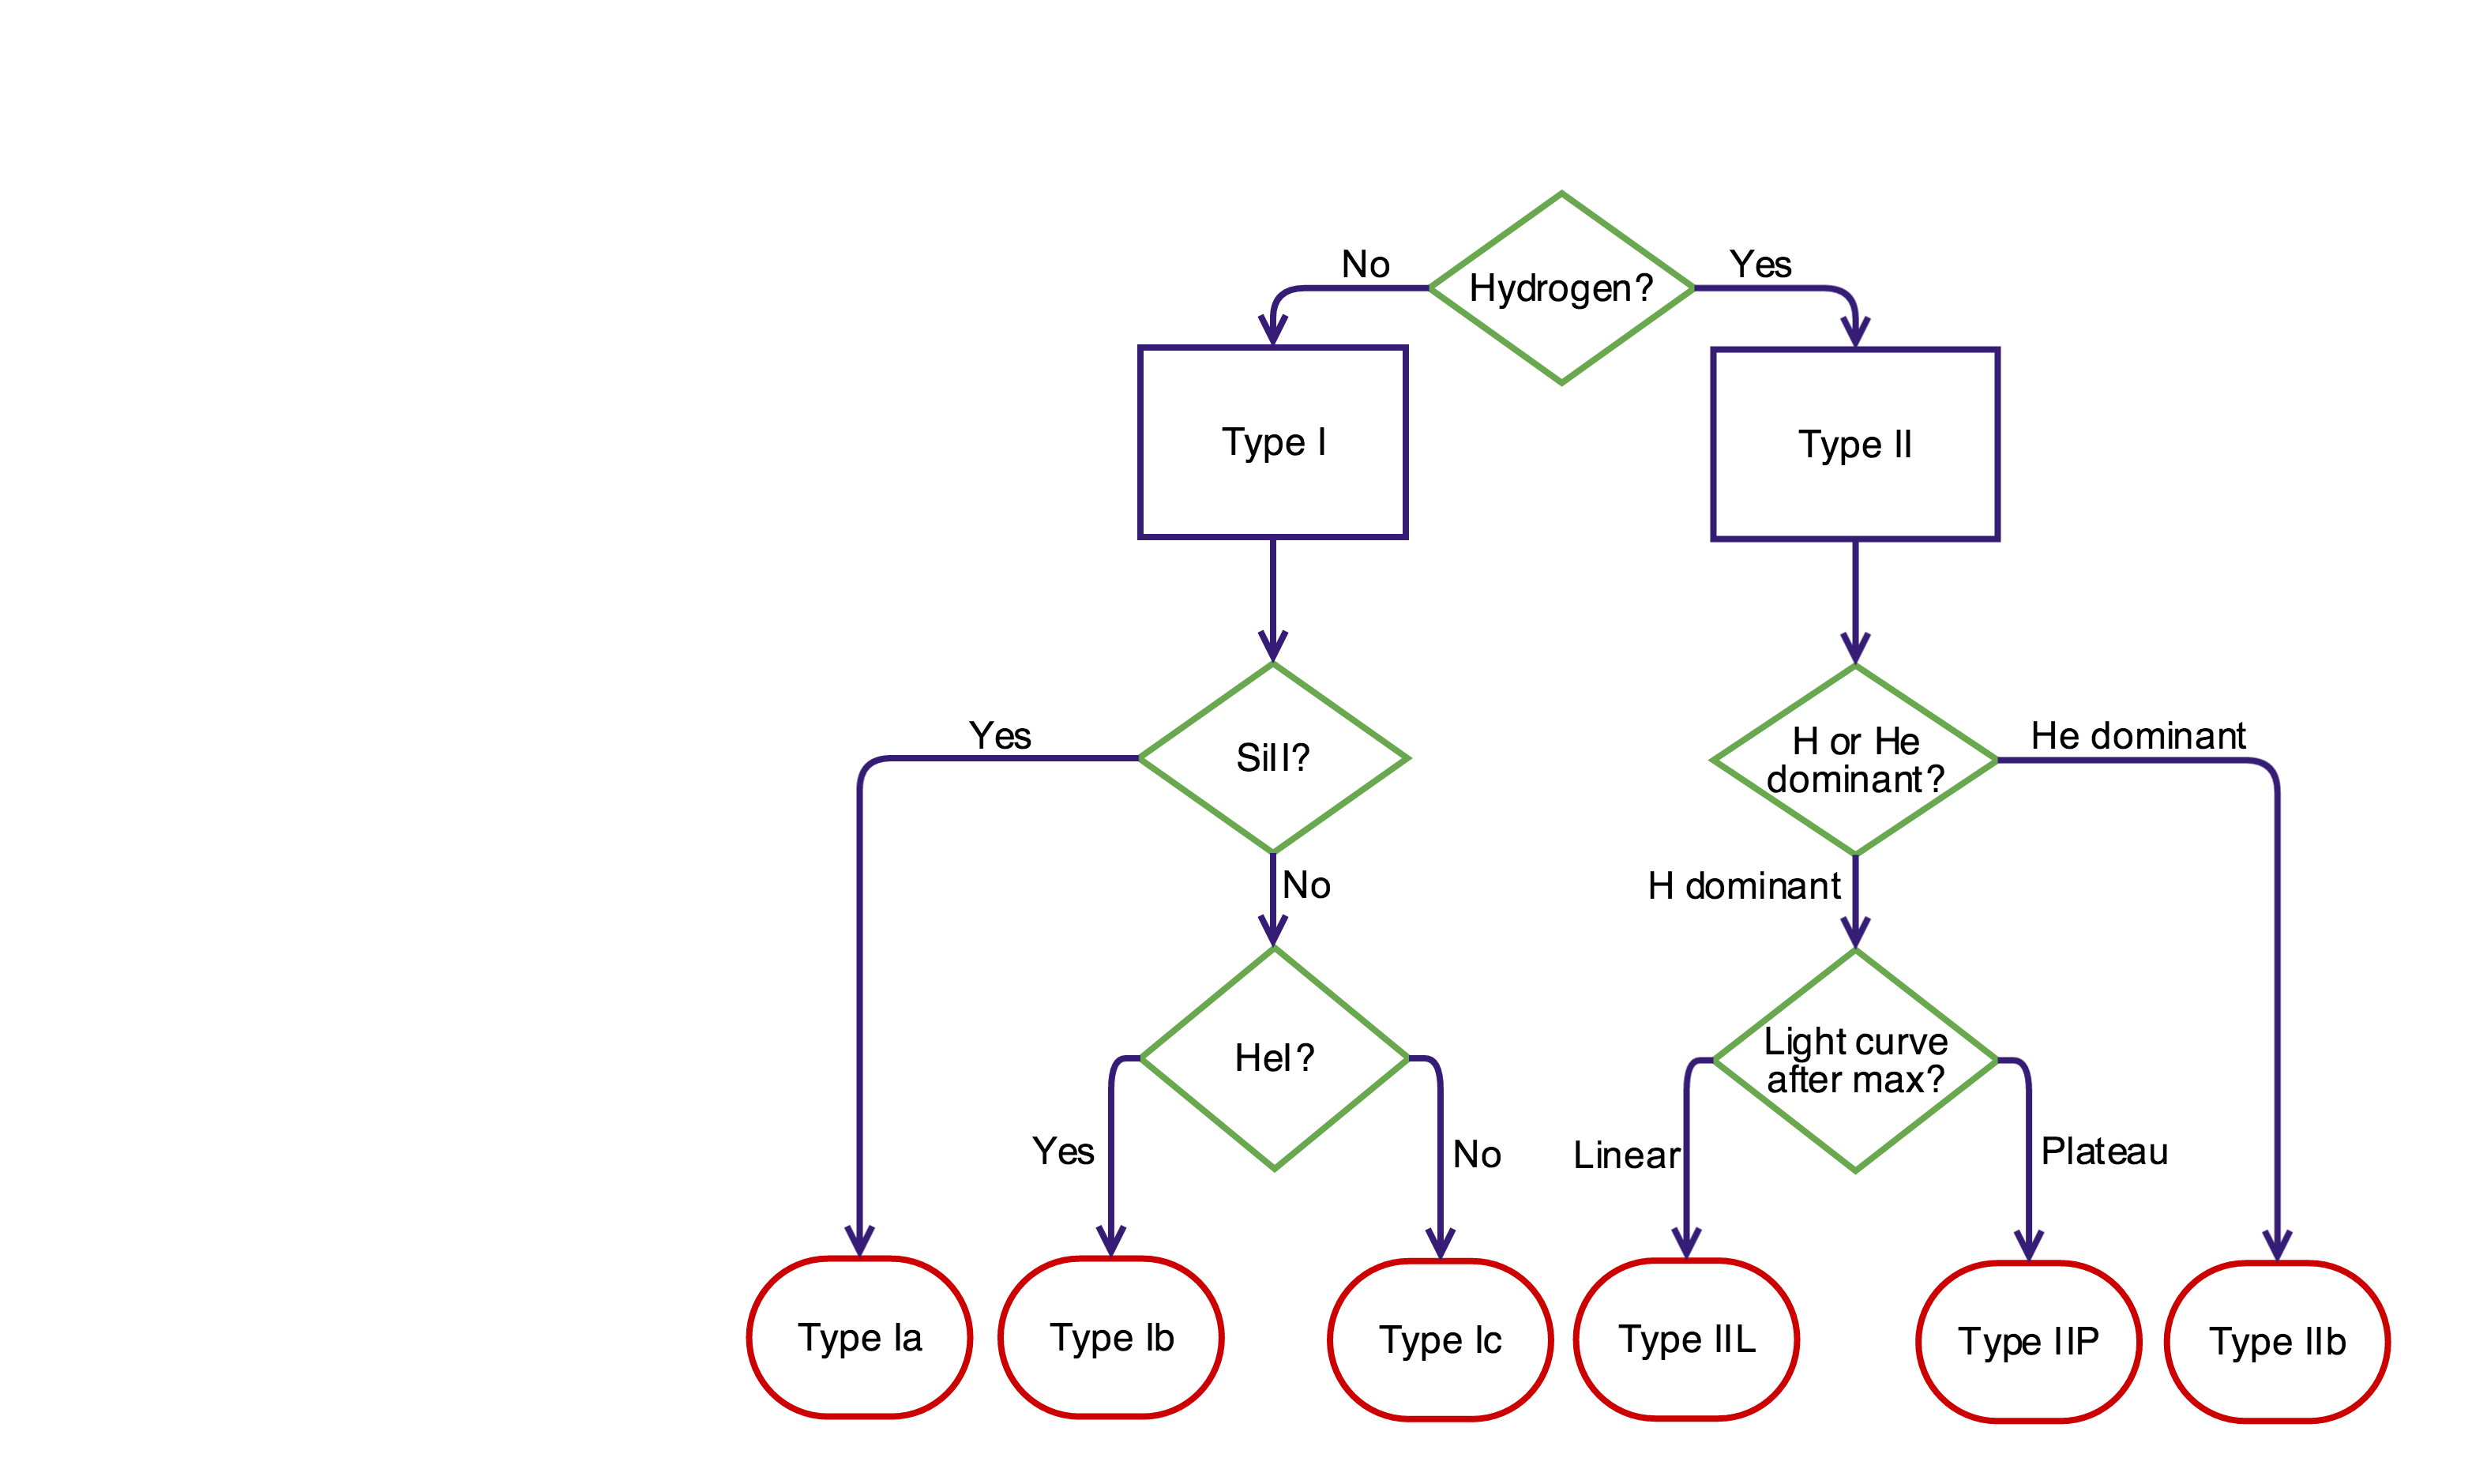
\includegraphics[clip=true, scale = 0.2, trim= 930 50 55 210]{chapters/chapter1/figs/sn_classification.png}
\caption{A flowchart summarising the supernova classification scheme}
\label{intro:fig:sn_class}
\end{figure}

\subsection{Types of Supernovae}

Supernovae may be classified into a number of different types.  They are bisected initially into Types I and II according respectively to the absence or presence of hydrogen in their early spectra.  Further sub-classifications depend on  other features in the early spectra, properties of later spectra and the evolution of the  light curve after maximum light.  A summary of the supernova classification scheme is presented in Figure \ref{intro:fig:sn_class}.  


If the initial classification is Type I then all further sub-classifications depend solely on the properties of the early spectra (a few days after outburst) as detailed in Figure \ref{intro:fig:sn_class}.  Type II supernovae are somewhat more complex in their categorisation.  After primary classification as a Type II SN, further subdivisions depend on the dominance of hydrogen or helium in \textit{later} spectra.  Helium dominant supernovae are classified as Type IIb and hydrogen dominant supernovae are classified as either Type IIL (those which have a linearly decaying light curve after maximum light) or Type IIP (those that exhibit a plateauing light curve after maximum light) as illustrated in Figure \ref{fig:light_curves}.  Type IIn supernovae are omitted from the summary presented in Figure \ref{intro:fig:sn_class} as they cannot be classified straightforwardly via a bifurcating process.  Type IIn supernovae will generally have strong emission lines, particularly hydrogen lines, often with complex profiles.  Crucially, the spectra of Type IIn supernovae do not exhibit the broad absorption features frequently seen in other types and instead contain narrow lines (hence Type IIn).  

\begin{figure}
\centering
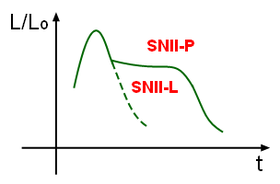
\includegraphics[clip=true, scale = 1, trim=0 0 0 0]{chapters/chapter1/figs/light_curves.png}
\caption{Illustration of the different shapes of light curves for Type IIP and Type IIL supernovae.}
\label{fig:light_curves}
\end{figure}

\subsection{From Massive Stars to Remnants}

It is now generally accepted that the progenitors of Type Ia supernovae are white dwarfs that exist in a binary system with another star \citep{Wang2012}.  The accretion of material from one star to another results in a thermonuclear explosion, a mechanism that is unique to Type Ia supernovae.  There have not been any observations suggestive of ejecta-condensed dust forming in the aftermath of a Type Ia supernova and I therefore do not consider these objects any further, focusing my attention solely on supernovae that explode via the core-collapse mechanism.  

Broadly, this process is initiated when a massive star ($\ge 8$M$_{\odot}$) starts to fuse heavier elements. The fusion of ever heavier elements generates increasingly less energy whilst also causing the mass of the core to increase.  Eventually, radiation pressure drops sufficiently that the core can no longer support itself against its own self-gravity and begins to collapse rapidly. Within milliseconds, the core reaches extremely high densities and, when it can no longer condense further, ``bounces" off itself causing  an immense shockwave to propagate outwards and a vast quantity of energy to be released via the expulsion of neutrinos.  Much of this complex process is still poorly understood and interesting models are currently being produced recreating these very early stages using a numerical approach \citep{Hammer2010,Takiwaki2014,Wongwathanarat2015}.  Though the explosion mechanisms of CCSNe are largely beyond the scope of my work, some attention will be paid to these models later in this thesis since instabilities that arise in these early stages can influence the structure of the ejecta at later stages of its evolution.

For many years after the explosion, the supernova (now a remnant) is in the free-expansion phase \citep{Landau1959,Ostriker1988}. During this phase, the mass and velocity of the expanding supernova massively exceed those of the surrounding medium, fortuitously allowing the behaviour of the SNR to be analysed as if it were expanding into a vacuum.  The shock radius during this phase may therefore be calculated simply as $R_s = v_s t$.  As the shockwave propagates through the ISM, interstellar material that has been compressed by the forward shock begins to accumulate.  At the same time a reverse shock wave begins to propagate back through the ejecta.  It is during this phase, which arises very soon after the initial explosion and typically lasts for a few hundred years, that the physical conditions in the ejecta are thought to be optimal for dust formation.  The phase ends when the mass of material ahead of the forward shock is of a similar magnitude to that behind and the mathematical treatment of its behaviour must be altered as it enters the Sedov-Taylor phase.
 
The Sedov-Taylor phase is pressure-driven and can be regarded as adiabatic, the gas cooling because of its expansion. The dynamics of this phase can also be described analytically but the derivation is slightly more complex than the free expansion phase \citep{Taylor1950,Sedov1959}.  Once a critical temperature is reached, ions start to recapture free electrons and energy is lost via radiation as the nebula starts to neutralise in what is known as the snow-plough phase, so called because the mass of swept-up material now greatly exceeds the ejected mass.  The expansion slows and eventually the shell breaks up into clumps and merges into the ISM.

 
 \subsection{Energetics in Core-Collapse Supernovae}

There are three different sources of energy in most supernovae.  Each of these emerges from the supernova in different forms over different timescales.  Initially, the most obvious energy source is that of the initial gravitational collapse which results in a huge emission of energy in the form of neutrinos and lasts for just a few seconds.  

The next source of energy to become apparent is that of the radioactive decay of unstable isotopes in the debris.  As these isotopes decay they produce gamma rays that Compton scatter off bound electrons.  This produces a population of fast, primary photoelectrons that cause further ionisations and excitations and produces a family of slower secondary electrons.  As these electrons recombine with ions and atoms become de-excited they emit monochromatic photons that we observe as line emission.  I will be particularly interested in those lines in the optical and IR, for example the Balmer and Paschen series of hydrogen lines are often prominent in the spectra of CCSNe (see Figure \ref{fig:balmer}).

 \begin{figure}
\centering
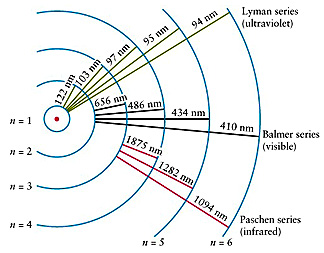
\includegraphics[clip=true,scale=0.9,trim= 0 0 0 0]{chapters/chapter1/figs/balmer1.jpg}
\caption{Illustration of the Lyman, Balmer and Paschen series of transitions in hydrogen.}
\label{fig:balmer}
\end{figure}


Finally, over much longer timescales, the kinetic energy of the expanding debris will emerge as radiation when it impacts the surrounding material.  This impact will propagate a reverse shock inwards through the ejecta and gas between the forward and reverse shocks will be heated and will therefore radiate its thermal energy as X-rays.  This stage of the energetics is likely coincident with the supernova remnant entering the Sedov-Taylor phase and so will usually only occur after several centuries.  

\subsection{Dust Formation and Destruction in CCSNe}
\label{scn:dust_formation}

The initial formation of dust grains requires high densities and low temperatures.  Although dust grains can grow via the accretion of individual atoms in the interstellar medium, various theoretical and experimental models indicate that dust grains cannot initially form via this process due to the low densities present \citep{Osterbrock2006}.  There are two primary theories for the formation of dust grains.  It was originally thought that the formation of dust grains resulted from the stochastic process of classical nucleation whereby particles coalesce to form the seeds of dust grains.  These seeds become the nucleation sites from which grains are ultimately born through the aggregation of further particles.  Various models of dust formation in the ejecta of CCSNe have used this approach \citep{Kozasa1989, Todini2001,Nozawa2003, Schneider2004}.  

More recently, several models of dust formation in CCSNe that consider the effects of chemistry on the growth of dust grains have been published.   These models consider the chemical composition of the gas and include chemical reaction rates thereby considering the manner in which molecular evolution influences dust grain formation and growth rates \citep{Cherchneff2009, Cherchneff2010, Sarangi2013, Sarangi2015}.  Models using both methods have predicted dust masses of the order of $0.1-1$M$_{\odot}$ of dust forming within the ejecta of CCSNe of progenitor masses between $12-40$M$_{\odot}$ within the first few years after the initial explosion.  

Whilst the issue of the quantities of dust that are initially produced in the ejecta of SNe is extremely important, another key question is what fraction of the dust that forms is capable of surviving to enter the interstellar medium at later times. Dust grains can be destroyed by a number of different processes.  Of primary interest is a process known as ``sputtering": collisions between dust grains and ions in a nebula can result in atoms or molecules being `knocked off' the surface of the grain.  Conditions for sputtering to occur are ideal near a shock-front \citep{Barlow1977} and it is therefore predicted that the passage of the reverse-shock back through the ejecta of a CCSN results in dust grains becoming fragmented into smaller grains or being destroyed entirely.  Understanding the initial grain size distribution and mass of the newly-formed dust in the ejecta is therefore extremely important to determining how much dust survives to enter the ISM and therefore whether CCSNe are in fact a significant source of dust in the universe.

%Talk more here about the quantities via each method - see Gomez review

\subsection{The Four Signatures of Dust in Core-Collapse Supernovae}
\label{three_sigs}

%POLARISATION = four.  Should include and also include reference to gomez review 2013.

The presence of dust in the ejecta of CCSNe can be indicated by four main signatures: 

\subsubsection{A decrease in the light curve} 
As the dust begins to form in the ejecta, UV and optical light is absorbed by the dust causing a decrease in the light curve at these wavelengths.  Whilst this signature indicates the presence of newly-forming dust, it is generally very difficult to use this signature to quantify properties of the dust.

\subsubsection{Excess IR emission}
An increase in emission in the IR occurs contemporaneously with the decrease in the UV-optical light curve.  A thermal MIR excess is caused by warm dust and an excess in the far-IR and sub-mm is the result of cold dust.  The increase in emission at these wavelengths can be caused by newly-formed dust condensing in the ejecta but can also be a result of the illumination of pre-existing dust.  This signature has been widely exploited using both radiative transfer models and blackbody fitting to derive properties of the dust from the observed SED \citep{Wooden1993}.

\subsubsection{Blue-shifted line profiles}
The onset of the formation of dust can cause an asymmetry in line profiles in the optical and IR.  The absorption and scattering of optical or near-IR radiation by newly-formed dust within the ejecta can result in an asymmetry between the red and blue shifted components, with redwards 
emission from the far side of the ejecta undergoing greater absorption and resulting in an overall shift of the profile to the blue.  This was first discussed by \citet{Lucy1989} and has been referenced qualitatively in the literature frequently, although it has not been used to quantitatively derive properties of the dust since that first publication by Lucy and collaborators.

\subsubsection{Polarised dust emission}
The expansion of a CCSNe is often somewhat asymmetrical and dust grain shapes are likely not spherical in shape.  Both of these factors can cause the emission from dust grains in the ejecta of supernovae to be highly polarised.  Analysis of the degree and orientation of the polarised emission can provide insight into the distribution and mass of the emitting dust.  This approach has only been applied to old remnants (the SCUBA polarimeter was used to isolate dust in the ejecta of Cas~A \citep{Dunne2009}) and has not yet been used for a supernova younger than $\sim$30 years.
\\

\noindent All four of these signatures have been discussed in detail over the timeline of this subject (e.g. \citet{Gomez2013}) but the focus has largely been on using the excess IR emission seen in the SED of CCSNe to determine quantitatively dust masses in these objects.  
%This approach has resulted in a lively debate regarding the quantities of dust that CCSNe are capable of producing.
 

\subsection{The Dust Mass Debate}

The formation of dust grains requires densities high enough for interaction between particles to take place, but temperatures that are cool enough to allow the grains to form and survive.  The theory that the ejecta of a CCSN in its free-expansion phase could provide these conditions  was first hypothesised by \citeauthor{Cernuschi1967} in 1967 and they have now long been thought to be potential dust factories \citep{Hoyle1970, Kozasa1991, Todini2001,Nozawa2003}.  The ejecta cools rapidly as it expands and there is an abundance of heavy elements.  In order to account for the large masses of dust seen in the early universe, it is estimated that CCSNe would need to produce  $0.1-1.0$M$_\odot$ of dust per CCSN  \citep{Morgan2003, Dwek2007}

Until recently, supernovae had been largely dismissed as a significant source of dust.  Observations over the last decade at mid-infrared (MIR) wavelengths of warm dust emission (200 - 450K)  from CCSNe had suggested that the quantities of ejecta-condensed dust produced during the first 1000 days were typically $\leq$ 10$^{-3}$~M$_\odot$  \citep{Sugerman2006, Meikle2007, Kotak2009, Andrews2010, Fabbri2011}.  This is much less than theoretical models predict (see Section \ref{scn:dust_formation}) and would not account for the dust masses observed in the early universe.  These observations indicated the need to find another early-time source of dust.

\subsubsection{Cassiopeia A}

In 2003, however, the field was shaken by the report that $2-4$M$_{\odot}$ of cold dust (20K) had been detected via sub-mm emission in the 300-year old SNR Cas~A using the Sub-millimetre Common-User Bolometer Array (SCUBA) \citep{Dunne2003}.   A heated debate followed as astronomers contested the source of the observed dust.  \citet{Dunne2003} had concluded that the dust was associated with the remnant based on the high spatial correlation of the sub-mm emission from the cold dust and the forward and reverse shocks that were traced via X-rays. \citet{Krause2004} refuted this suggestion using analyses of the line emission and absorption to conclude that the dust was in fact located in clouds along the line of sight to the remnant.  A determination was sought by considering the polarisation of the dust emission.  As discussed in the previous section, the asymmetric nature of expansion likely results in a degree of polarisation relative to stationary dust located in the ISM.  Observations of Cas~A in the sub-mm were made using the SCUBA polarimeter and the emission was found to be extremely polarised to a fraction of 30\% (compared to typical ISM fractions of 2\% - 7\%).  A reevaluation of the dust mass based only on the polarised emission  estimated the mass of dust in Cas~A to be ~1M$_{\odot}$ \citep{Dunne2009}.

\begin{figure}
\centering
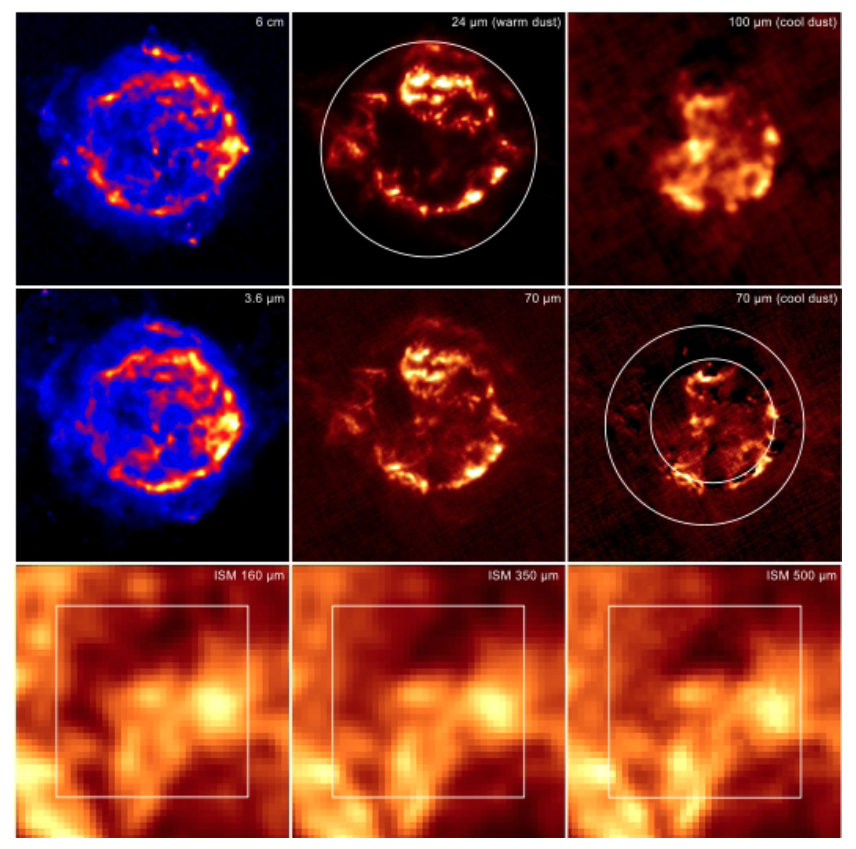
\includegraphics[clip=true,scale=0.425,trim= 0 0 0 0]{chapters/chapter1/figs/CasA.png}
\caption{Images of Cas~A at IR, sub-mm and radio wavelengths.  The top six images are 7' on a side and the bottom three are 10' on a side.  The inner and outer circles in the middle-right image correspond to the reverse and forward shocks respectively according to \citep{Gotthelf2001}.  Image taken from \citet{Barlow2010}.}
\label{fig:CasA}
\end{figure}


Even this revised estimate was still uncomfortably large compared to previous estimates.  Sadly, SCUBA was taken offline shortly after this observation and so follow-up observations of Cas~A and other remnants using SCUBA were not possible.  It was only with the advent of the \textit{Herschel} mission that the presence of cold dust in SNRs could again be investigated via emission in the sub-mm.  These \textit{Herschel} observations have, somewhat surprisingly for many in the field, consistently revealed dust masses of the order of $0.1-1.0$M$_{\odot}$ in a number of SNRs.

%Critical to the investigation of dust formation in SNRs in recent years have been a few key objects, namely Cas~A, the Crab nebula and SN~1987A.  As a central focus of this thesis, I will discuss the history of SN~1987A and dust formation within its ejecta in detail at the start of Chapter \ref{chp:chp5} and so I limit my discussion here to just Cas~A and the Crab nebula. 

%By 2009, large masses of dust had been detected in Cas~A using SCUBA.  

As the first result of its kind, and with a great many questions left unanswered, it was crucial to establish the dust mass in Cas~A as conclusively as possible.   Observations of Cas~A using \textit{Spitzer} detected emission from warm dust between 24$\mu$m - 70$\mu$m, analysis of which established a dust temperature of 60 - 120K and a dust mass of 0.02 - 0.054M$_{\odot}$ \citep{Rho2008}.  Subsequent observations using \textit{Herschel} detected a cool dust component of ~0.075M$_{\odot}$ giving a total dust mass in Cas~A of $\sim$0.1M$_{\odot}$ \citep{Barlow2010}.  Like many {\em Herschel} observations, it is difficult to conclusively determine the location of the dust as within the remnant rather than in clouds in the foreground or background.  Images of Cas~A across a range of wavelengths are presented in Figure \ref{fig:CasA}.  

\subsubsection{The Crab Nebula}

The Crab nebula was first detected by Chinese astronomers in 1054.  A pulsar at the heart of the nebula illuminates the surrounding gas and dust and provides a rare opportunity to probe dust masses in a centuries old remnant.  Unlike Cas~A, the Crab does not have contaminating clouds of dust in its foreground and background ensuring that any detections of dust from this location are likely to be associated with the remnant.
 
\textit{Spitzer} and \textit{Herschel} observations have been made of this remnant and both have detected dust in the ejecta.  {\em Spitzer}, however, only detected $2.4\times10^{-3}$M$_{\odot}$.  Further spectroscopic and photometric observations with {\em Spitzer}, {\em Herschel} and Planck allowed the full range of the SED to be investigated and allowed for synchrotron and line emission to be well-characterised.  Subtracting this from the continuum observations yielded two dust components, a warm component at 63K estimated to have a mass of $\sim10^{-3}$M$_{\odot}$ and a cool component at  34K with an estimated mass of $0.1 - 0.2$M$_{\odot}$ \citep{Gomez2012,Temim2012}.  As might be expected, the dust is predominantly co-located with the gas in dense filaments (see Figure \ref{fig:Crab}).
 
 These dust masses were based on a two-component dust fitting.  Further analyses and models of these results have resulted in revised estimates of the mass of dust in the Crab nebula.  Multi-component fitting with multiple grain sizes by \citet{Temim2013} gave rise to a dust mass estimate of $0.02-0.13$M$_{\odot}$, consistent with the lower end of the previous estimate.  However, recent radiative transfer models by \citet{Owen2015} that account for varying grain size distributions, gas geometries and a more realistic heating source derive dust masses consistent with the estimated $0.1-0.2$M$_{\odot}$ of \citet{Gomez2012}.  If the dust in the ejecta is assumed to be clumped however, as is likely more realistic, then $0.4 - 0.6$M$_{\odot}$ of amorphous carbon grains are required to fit the SED.  At this time, the Crab nebula was the only object to have provided a clean view of large masses of dust ($>10^{-3}$M$_{\odot}$) in a SNR .
 
 \begin{figure}
\centering
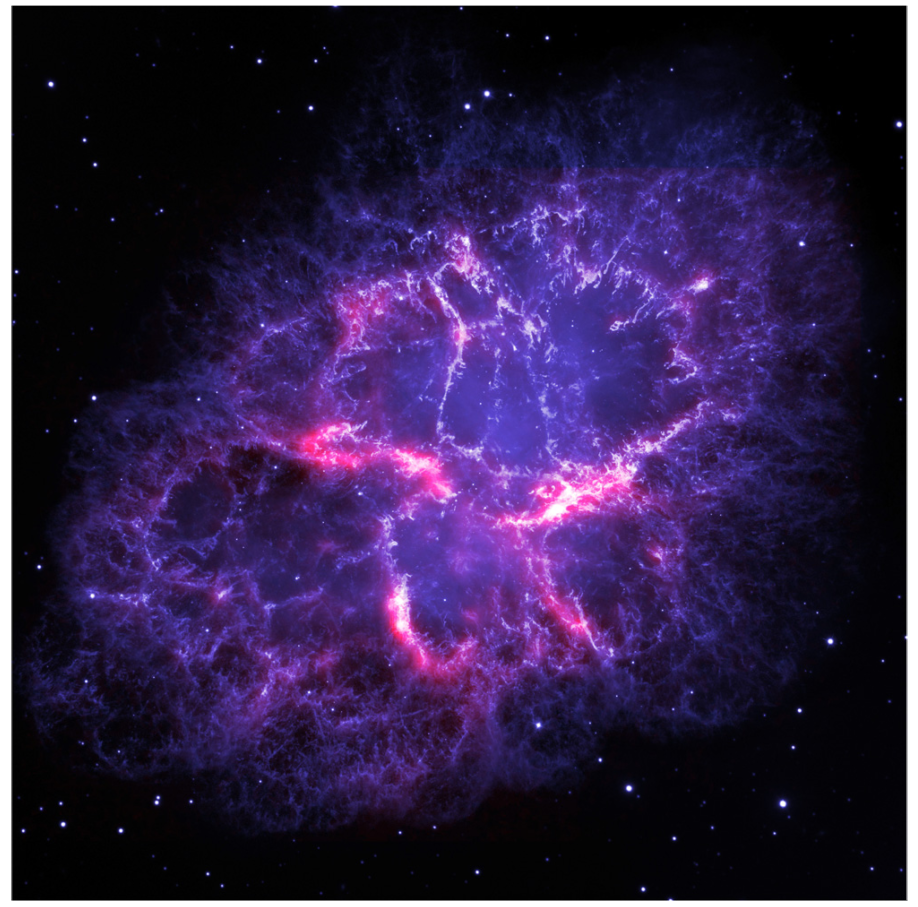
\includegraphics[clip=true,scale=0.3,trim= 0 0 0 0]{chapters/chapter1/figs/Crab.png}
\caption{Composite image of the Crab nebula using Hubble Space Telescope (HST) optical line emission data (blue-white) and {\em Herschel} 70$\mu$m dust emission (red) illustrating the close alignment between the optical knots and filaments.  Credits: Oli Usher (UCL); \textit{Herschel Space Observatory, Hubble Space Telescope}: ESA, NASA.  Image taken from \citet{Owen2015}.}
\label{fig:Crab}
\end{figure}
 
 \subsubsection{SN~1987A}
 
 Perhaps the most critical discovery however, was that of dust in the ejecta of SN~1987A.  This object is uniquely helpful in the study of supernovae due its location only $\sim$50kpc away.  Dust had long been theorised in the ejecta of SN~1987A but only in comparatively small quantities.  Observations of blue-shifted line profiles in the optical and of warm dust emission in the MIR confirmed this hypothesis with dust mass estimates of $\sim5\times 10^{-4}$M$_{\odot} - 2 \times 10^{-3}$M$_{\odot}$ forming in the first 1000 days \citep{Lucy1989,Roche1989,Bouchet1991,Wooden1993,Ercolano2007}.  In 2010, this view was fundamentally altered by observations by \textit{Herschel} that indicated the presence of $0.4-0.7$M$_{\odot}$ of cold dust.  Further observations with {\em Herschel} and the Atacama Large Millimetre Array (ALMA) not only confirmed this dust mass estimate but also had sufficient spatial resolution to conclusively determine the origin of the cold dust emission as from within the ejecta \citep{Matsuura2011,Indebetouw2014,Matsuura2015}.  Recent modelling of the evolution of the optical and IR SED has predicted similarly large  masses of cold dust to  have formed in the ejecta of SN~1987A, with the majority of the dust forming after 1000 days \citep{Wesson2015}.
 
 This object is crucial to the field and is a central focus of this thesis.  I have therefore only elucidated the key points above and will give a considerably more detailed synopsis of the story of SN~1987A at the start of Chapter \ref{chp:chp5}.
 
\vspace{3ex}
\noindent These recent {\em Herschel} far-IR and sub-mm observations of several SNRs have revealed cold dust masses as high as $0.2-0.8$M$_{\odot}$.  These discoveries have resulted in a re-evaluation of the rate of dust production by CCSNe and a renewed focus on these objects as sources of dust.

However, there remain a large number of outstanding challenges to consider.  Firstly, there are still only a very small number of supernovae that have been observed to have sizeable masses of dust present in their ejecta.  If further CCSNe were also shown to have formed large quantities of dust then the already shifting opinion might start to become consensus.  Other points to consider regarding dust formation and evolution in CCSNe include the nature of the dust (composition, grain size, grain shape etc.) which is still largely unclear, as is the extent to which it is destroyed or sputtered after its initial formation.  Related to these issues is the uncertainty of the dust formation rate in the ejecta and the issue of where this formation takes place.  These are all interesting questions that call out for answers.  

 \subsection{Observations of Dust-Affected Asymmetric Line Profiles}

The {\em Hershel} dust mass estimates were based on fitting dust SEDs that peaked at far-IR wavelengths. Unfortunately, following the end of the {\em Herschel} mission in 2013, there is likely to be a long wait for far-IR facilities with comparable or better sensitivities than {\em Herschel} to become available.  Without data, this methodology is temporarily ineffectual.  This has provided an incentive to make use of alternative methods to estimate the dust masses that form in supernova ejecta.

\begin{figure}
\centering
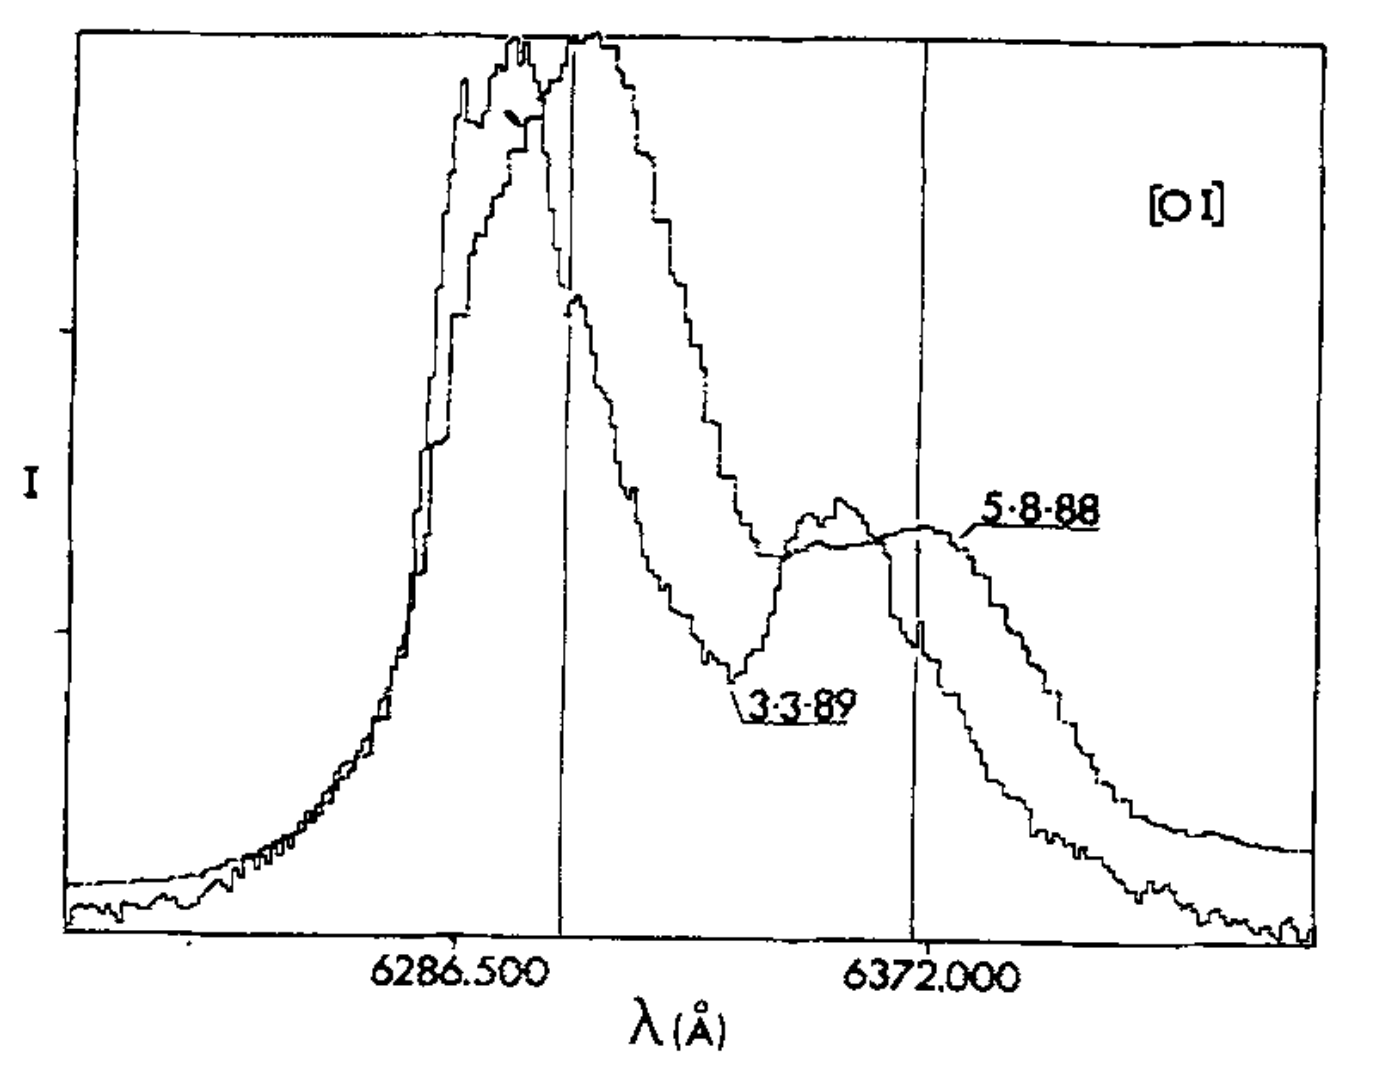
\includegraphics[clip=true,scale=0.45,trim= 0 0 0 0,angle=1]{chapters/chapter1/figs/LucyOI.png}
\caption{The emission profile of [O~{\sc i}]$\lambda$6300,6363~\AA\ from SN~1987A on 5 August 1988 (day 529) and 3 March 1989 (day 739) showing the strong blue-shift by $\sim600 $~km~s$^{-1}$ of the latter profile.  The profiles are scaled to the same peak intensity for the violet component.  The image is taken from \citet{Lucy1989}.}
\label{fig:Lucy_orig}
\end{figure}


As discussed in Section \ref{three_sigs}, there is more than one way of tracing dust formation in the ejecta of supernovae.  In 1989, \citeauthor{Lucy1989} identified a progressive blue-shifting of the [O~{\sc i}]~$\lambda$6300,6363~\AA\ doublet from SN~1987A between days 529 and 739 after outburst, with the doublet in the later spectrum being blue-shifted by $\sim600 $~km~s$^{-1}$ (see Figure \ref{fig:Lucy_orig}). Since then, such red-blue asymmetries have been frequently observed in the late-time ($ > 400$ days) spectra of supernova ejecta  .

Numerous telescopes have recorded spectra of CCSNe in the optical and IR, some with extremely high resolution.  The Anglo-Australian Telescope (AAT), the Cerro Tololo Inter-American Observatory (CTIO), the Hubble Space Telescope (HST) and the Very Large Telescope (VLT) have all observed several supernovae in the optical including SN 1987A.  Other telescopes such as the two Gemini Multi-Object Spectrographs (GMOS) have also taken spectra of numerous CCSNe.  As a result of observations with these telescopes, numerous CCSNe have been observed to exhibit the blue-shifted line profiles indicative of dust formation in the ejecta (e.g. \citet{Lucy1989,Fabbri2011,Mauerhan2012,Milisavljevic2012}).  A recent example of such is given in Figure \ref{fig:2010jl} which illustrates the progressive blue-shifting of the line profiles of H$\alpha$, H$\beta$ and  HeI $\lambda$5876\AA\ from SN~2010jl \citep{Gall2014}.

Advances in digital storage have allowed for spectral and photometric observations to be made  available online.  Many observatories now publish their recent observations online in archives and are working to upload observations that pre-date file sharing services and so there is now a growing database of dust-affected asymmetric line profiles easily available. Much of the data used in this thesis was obtained from these archives.
\begin{figure}[!t]
\centering
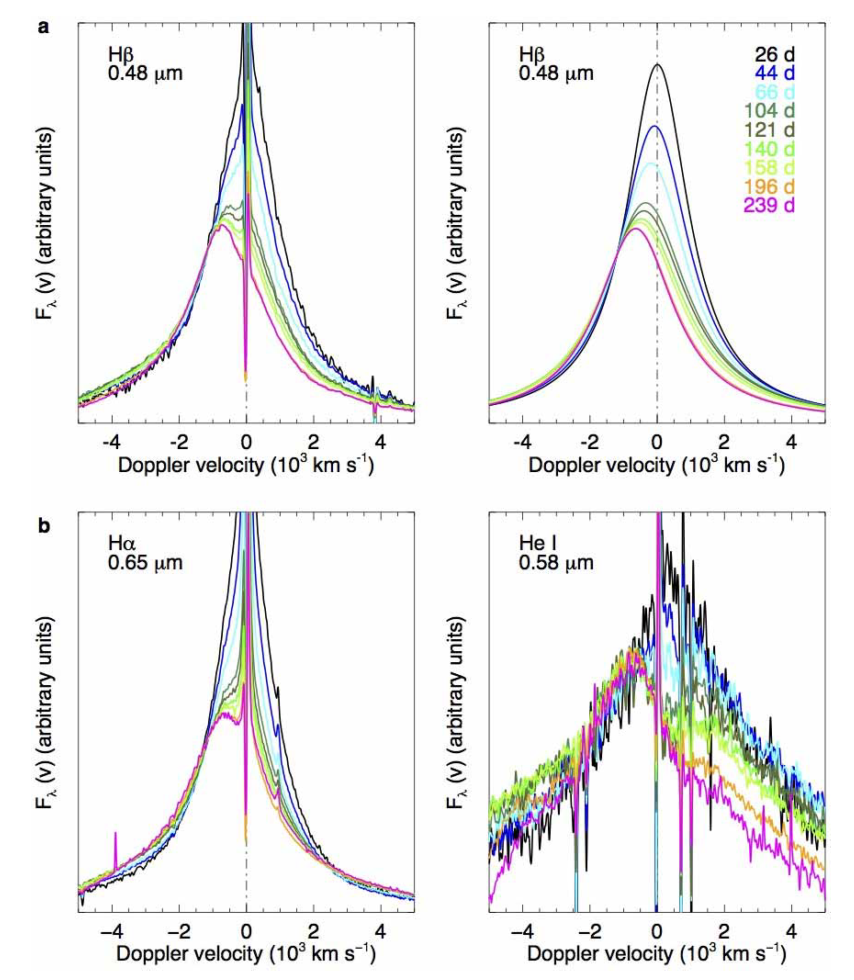
\includegraphics[clip=true,scale=0.4,trim= 0 -20 0 -20]{chapters/chapter1/figs/2010jl.png}
\caption{Figure taken from \citet{Gall2014} illustrating the progressive blue-shifting of line profiles from SN~2010jl.  {\em a.} Evolution of the H$\beta$ line profile {\em (left)} and Lorentzian line fits to this line {\em (right)}. {\em b.} Evolution of the H$\alpha$ line {\em (left)} and the He{\sc i} $\lambda$5876\AA\ line {\em (right)}.}
\label{fig:2010jl}
\end{figure}



%Talk about the various observations of the red-blue asymmetry

Quantitative modelling of the extent of this asymmetry and other aspects of the shape of the line profile allow for dust in the ejecta of supernovae to be traced via an alternative method to SED-fitting.  







\section{Aims and Content Of This Thesis}
The purpose of my work has been to develop a new approach to determining dust masses in supernovae, with the aim of providing an alternative to SED fitting for the future and of corroborating or contradicting past dust mass estimates.  I looked to exploit the dust-forming signature of characteristically asymmetric line profiles.  Though this feature has been discussed at length by numerous authors, it has very rarely been quantitatively measured or modelled.

To this end, I have developed a Monte Carlo  code that numerically models this signature in the spectra of CCSNe in order to quantitatively determine dust masses formed at a variety of epochs post-explosion, additionally seeking to place constraints on the composition and grain size distributions of the newly-formed dust. I have sought to use this new code to model the dust mass evolution  of SN~1987A and the dust masses present at late times in a number of other supernovae.  I hope ultimately to have presented a convincing picture of the efficacy of CCSNe as the birthplaces of large masses of dust.

In Chapter \ref{chp:chp2}, I will detail the physics that is included in DAMOCLES and the mechanisms and algorithms behind the functioning of the code.  I will also discuss technical details and the motivations behind various choices such as the use of the Monte Carlo methodology and the use of the Fortran 95 programming language.  

In Chapter \ref{chp:chp4}, I will describe the process of testing the code.  I will detail the algebraic derivation of analytical line profiles in optically thin regimes and consider previous work published on line profiles in optically thick environments.  I will demonstrate that DAMOCLES is capable of reproducing these results before moving on to present an investigation of the variable parameter space from a theoretical perspective.  By probing the effects on the line profile of varying a single parameter, I discovered a number of interesting features that are caused by dust scattering and absorption.  These are also discussed in Chapter \ref{chp:chp4}.  

I used DAMOCLES to number a model of CCSNe with a particular focus on SN~1987A.  For many reasons this object became the central focus of this thesis. The detailed models of the H$\alpha$ and [O~{\sc i}]$\lambda$6300,6363~\AA\ from SN~1987A over a wide range of epochs and a discussion of the implications of my results are presented in Chapter \ref{chp:chp5}.  

Chapter \ref{chp:chp6} contains models of some late-time line profiles from a number of other CCSNe, namely SN~1980K, SN~1993J and Cas~A.  I discuss my models of a variety of oxygen and hydrogen lines and their implications for dust formation in CCSNe in general.  Finally, I will bring together my findings and conclude this thesis in Chapter \ref{chp:chp7}.

